\documentclass{article}
\usepackage[utf8]{inputenc}
\usepackage{amsmath}
\usepackage{geometry}
\geometry{
 a4paper,
 total={182mm,257mm},
 left=14mm,
 top=20mm,
 }
 \usepackage[utf8]{inputenc}
 \usepackage[italian]{babel}
\usepackage[T1]{fontenc}
\usepackage{amssymb}
\usepackage{physics}
\usepackage{tikz} 
\usepackage{graphicx}
\graphicspath{ {Immagini/} }
\usepackage{float}
\usepackage{hyperref}
\hypersetup{
    colorlinks=true,
    linkcolor=red,
    citecolor=green
    filecolor=magenta,      
    urlcolor=cyan,
}


%Theorem Environments
\newtheorem{thm}{Teorema}[section]
\newtheorem{lem}[thm]{Lemma}
\newtheorem{property}{Proprietà}[section]
\newtheorem{defn}{Definizione}[section]
\newtheorem{prop}[defn]{Proposizione}
\newtheorem{example}{Esempi}[subsection]
\newtheorem{exerc}[example]{Esercizi Svolti}

%Commandi di Formattazione
\newcommand{\noi}{\noindent}
\newcommand{\note}{\noindent {\quad \bf \underline{Osservazione:}} \quad}
\newcommand{\eg}{\noindent {\bf \underline{Esempio:}} \quad}
\newcommand{\bfemph}[1]{\textbf{\textit{#1}}}
\renewcommand{\emph}[1]{\bfemph{#1}}

%Number Sets
\newcommand{\R}{\mathbb{R}}
\newcommand{\C}{\mathbb{C}}
\newcommand{\Z}{\mathbb{Z}}
\newcommand{\Q}{\mathbb{Q}}

%Shortcuts
\newcommand{\then}{\ensuremath{\Rightarrow}}
\newcommand{\twopartdef}[4]
{
	\left\{
		\begin{array}{ll}
			#1 & \mbox{se } #2 \\
			#3 & \mbox{se } #4
		\end{array}
	\right.
}

%Vectors
\renewcommand{\i}{\vu{i}}
\renewcommand{\j}{\vu{j}}
\renewcommand{\k}{\vu{k}}
\renewcommand{\a}{\va{a}}
\renewcommand{\b}{\va{b}}
\renewcommand{\c}{\va{c}}
\renewcommand{\v}{\va{v}}
\renewcommand{\u}{\va{u}}
\newcommand{\s}{\va{s}}
\renewcommand{\t}{\va{t}}
\newcommand{\verst}{\vu{t}}
\newcommand{\versr}{\vu{r}}
\renewcommand{\r}{\va{r}}
\newcommand{\tauvs}{\vu{\tau}}
\newcommand{\tauvt}{\va{\tau}}
\newcommand{\normvs}{\vu{n}}
\newcommand{\N}{\va{N}}
\newcommand{\g}{\va{g}}
\newcommand{\F}{\va{F}}
\newcommand{\f}{\va{f}}
\newcommand{\M}{\va{M}}
\renewcommand{\l}{\va{l}}
\newcommand{\p}{\va{p}}
\renewcommand{\P}{\va{P}}
\renewcommand{\L}{\va{L}}

\title{Appunti Lezioni}
\author{Roberto Gargiulo}
\date{Ultimo Aggiornamento: \today}


\begin{document}

\maketitle


\section{Potenza, Lavoro ed Energia }
\begin{defn}
La \textbf{potenza} sviluppata da una forza $\F$ si definisce come il prodotto scalare tra la forza $\F(t)$ e la velocità $\v(t)$:
\[W(t)=\F(t)\cdot\v(t)\]
\end{defn}

\begin{thm}[Il Teorema delle Forze Vive]
Data una forza $\F$ applicata ad un corpo che si muove di velocità $\v(t)$, la potenza sviluppata dalla forza vale:
\begin{equation}
\begin{split}
    W(t)=\F(t)\cdot\v(t)&=m\dv{\v(t)}{t}\v(t)=\\
    &=m\frac{1}{2}\dv{\v(t)\cdot\v(t)}{t}=\frac{1}{2}m\dv{|\v(t)|^2}{t}=\\
    &=\boxed{\dv{t}\left(\frac{1}{2}mv^2\right)}
\end{split}    
\end{equation}
Definiamo la quantità $\frac{1}{2}mv^2$ \textbf{energia cinetica} K di un corpo di massa m che si muove con velocità di modulo v.
\end{thm}
\begin{defn}
Il \textbf{lavoro} compiuto dalla forza $\F$ in un intervallo $\Delta t=t_2-t_1$ si definisce come:
\begin{equation}
    \mathbb{L}(t_1,t_2)=\int_{t_1}^{t_2}W(t)\dd t=\int_{t_1}^{t_2}\F(t)\cdot\v(t)\dd t
\end{equation}
\end{defn}
\begin{thm}[Il Teorema del Lavoro e dell'Energia Cinetica]
Per il teorema della forze vive possiamo esplicitare la potenza sviluppata da $\F$ come derivata dell'energia cinetica rispetto al tempo:
\begin{equation}
    \mathbb{L}(t_1,t_2)=\int_{t_1}^{t_2}W(t)\dd t=\int_{t_1}^{t_2}\dv{K(t)}{t}\dd t=\int_{t_1}^{t_2}\dd K=K(t_2)-K(t_1)=K_2-K_1=\Delta K
\end{equation}
Ossia il lavoro compiuto da una forza implica una variazione di energia.
\end{thm}
\paragraph{Formulazione Alternativa del Lavoro}
Notiamo che esplicitando il lavoro secondo la sua definizione e a sua volta esplicitando la velocità come derivata del raggio vettore siamo in grado di ricondurre la definizione di lavoro come integrale di Riemann della potenza rispetta al tempo ad un integrale di linea della forza rispetto alla traiettoria:
\[\mathbb{L}(t_1,t_2)=\int_{t_1}^{t_2}W(t)\dd t=\int_{t_1}^{t_2}\F(t)\cdot\v(t)\dd t=\int_{t_1}^{t_2}\F(t)\cdot\dv{\r}{t}\dd t=\int_{P_1}^{P_2}\F(\r)\dd\r\]
Ponendo $P_1=\r(t_1),P_2=\r(t_2)$ e riscrivendo $\F$ in funzione di $\r$ invece che di t.
Possiamo inoltre ricondurre nuovamente questo integrale ad uno di Riemann ricordando la definizione di prodotto scalare in $V_3$:
\[\mathbb{L}(t_1,t_2)=\int_{P_1}^{P_2}\F\cdot\dd\r=\int_{P_1}^{P_2}|\F|\cos\alpha(s)|\dd \r|=\int_{P_1}^{P_2}|\F(s)|\cos\alpha(s)\dd s\]
Dove $s(t)$ è l'ascissa curvilinea, che si può invertire ($t=t(s)$)in modo da poter scrivere anche $\F$ in funzione di $s(t)$.
Le differenze principali tra queste formulazioni sono i diversi usi, la prima è più comoda da trattare analiticamente ed è utile quando è nota la velocità/posizione istante per istante mentre la seconda - sebbene più complicata - è particolarmente utile quando tutto ciò che è noto è la traiettoria e la forza in funzione di essa. Un esempio tipico è quello del lavoro fatto dalla tensione di un pendolo (non necessariamente semplice), in quanto siccome per le proprietà della circonferenza lo spostamento è perpendicolare alla tensione (radiale) in ogni punto allora ogni lavoro infinitesimo è nullo:
\[\dd\mathbb{L}=\tauvt\cdot\dd\r=0\then \mathbb{L}=\int\dd\mathbb{L}=0\]
\paragraph{Il Lavoro di più Forze}
Data la risultante delle forze $\F$:
\[\F=\F_1+\F_2+\F_3\]
Possiamo ottenere il lavoro esercitato dalla forza F come somma dei lavori esercitati da ciascuna forza:
\[\mathbb{L}=\int_{P_1}^{P_2}\F\dd\r=\int_{P_1}^{P_2}\left(\F_1+\F_2+\F_3\right)\dd\r=\int_{P_1}^{P_2}\F_1\dd\r+\int_{P_1}^{P_2}\F_2\dd\r+\int_{P_1}^{P_2}\F_3\dd\r=\mathbb{L_1}+\mathbb{L_2}+\mathbb{L_3}\]

\section{Campi di Forza}
\begin{defn}
Un \textbf{Campo di Forze} è una funzione $\F(\r)$ che associa ad ogni punto di una certa zona dello spazio un vettore $\F(\r)$.
\end{defn}
\begin{example}
Un esempio tipico è il campo gravitazionale che, nelle nostre approssimazioni, è uniforme (nello spazio) e costante (nel tempo).
\end{example}
Nei campi di forze ha senso quindi parlare di \textbf{lavori virtuali}, ossia il lavoro compiuto dalla forza $\F$ su una certa traiettoria $\gamma'$ contenuta nella parte di spazio su cui è definito il campo vettoriale. In generale il lavoro virtuale di una traiettoria immaginaria è ben distinto dal lavoro effettivo, ma esistono particolari campi di forze in cui non è cosi.
\begin{defn}
Un \textbf{Campo di Forze Conservativo} è un campo tale che dati due punti $P_1,P_2$ allora il lavoro compiuto dalle forze su una qualunque traiettoria che collega tali punti è lo stesso:
\[\int_\gamma\F(\r)\dd\r=\int_{\gamma'}\F(\r)\dd\r\]
\end{defn}
Questa proprietà permette quindi di non dover conoscere la traiettoria scelta dal corpo, in quanto note le posizioni di partenza e d'arrivo è possibile scegliere una qualunque traiettoria (quindi la più comoda per i calcoli) ottenendo lo stesso risultato. Osserviamo inoltre che per le proprietà degli integrali e dei campi conservativi il lavoro svolto su una curva chiusa è sempre nullo:
\[ {}_{\gamma_1} \int_{P_1}^{P_2}\F(\r)\dd\r={}_{\gamma_2} \int_{P_1}^{P_2}\F(\r)\dd\r=-{}_{\gamma_2} \int_{P_2}^{P_1}\F(\r)\dd\r\then {}_{\gamma_1}\int_{P_1}^{P_2}\F(\r)\dd\r+{}_{\gamma_2} \int_{P_2}^{P_1}\F(\r)\dd\r=0 \]
Ciò equivale alla scrittura seguente, che esprime un integrale di linea lungo una curva chiusa:
\begin{equation}
    \boxed{{}_\gamma\oint\F(\r)\dd\r=0}
\end{equation}
Grazie a queste proprietà è possibile definire il lavoro come funzione dei soli punti $P_1,P_2$, a sua volta esprimibile come differenza di una certa funzione $U$ nel punto $P_1$ e nel punto $P_2$:
\[\mathbb{L}=\int_{P_1}^{P_2}\F(\r)\dd\r=V(P_1,P_2)=U(P_1)-U(P_2)=-\Delta U\]
Possiamo quindi definire la \textbf{variazione di energia potenziale} come l'opposto del lavoro necessario a spostare un corpo da una posizione $P_1$ ad una posizione $P_2$. Inoltre, similmente al lavoro, la variazione di energia totale è data dalla somma delle variazioni di energia totali:
\[\Delta U=-\mathbb{L}=-(L_1+L_2+L_3)=-L_1-L_2-L_3=\Delta U_1+\Delta U_2+\Delta U_3\]

\section{Energia Meccanica}
Consideriamo il lavoro compiuto dalla risultante delle forze su un certo corpo, notiamo che siccome possiamo scrivere:
\[\F=\F^C+\F^{NC}\]
Ossia la risultante delle forze è data dalla risultante delle forze conservative e non conservative. Possiamo scrivere quindi:
\[\mathbb{L}=\mathbb{L}^C+\mathbb{L}^{NC}\]
Per definizione di energia potenziale e per il teorema dell'energia cinetica otteniamo quindi:
\[\Delta K=-\Delta U+\mathbb{L}^{NC}\]
Che si può riscrivere come:
\[\Delta K+\Delta U=\Delta(K+U)=\mathbb{L}^{NC}\]
Definiamo quindi la somma di energia cinetica e potenziale l'\textbf{energia meccanica} di un corpo ottenendo l'enunciato del \textbf{Teorema Generale delle'Energia Meccanica}:
\begin{thm}
\begin{equation}
    \boxed{\Delta E=\mathbb{L}^{NC}}
\end{equation}
\end{thm}
Che nel caso in cui un corpo è soggetto solo a forze conservative oppure le forze non conservative sono a lavoro nullo (ossia del tipo $\F\perp\dd\r$) otteniamo la \textbf{Conservazione dell'Energia Meccanica}:
\begin{equation}
    \Delta E=0\iff E_1=E_2
\end{equation}
Notiamo inoltre che per la definizione di energia potenziale, la funzione $U(\r)$ è determinata a meno di una costante $c$ la quale è fissata scelto lo zero dell'energia potenziale (solitamente quando la forza responsabile del campo si annulla). 
Consideriamo quindi il lavoro infinitesimo, detto \textbf{forma differenziale}:
\[\dd L=\F(\r)\dd\r=F_x\dd x+F_y\dd y+F_x\dd z\]
Mentre la variazione infinitesima di energia potenziale si può dimostrare valere:
\[\dd U=\pdv{U}{x}\dd x+\pdv{U}{y}\dd y+\pdv{U}{z}\dd z\]
Per un campo conservativo si verifica quindi:
\[\dd \mathbb{L}=-\dd U\]
In termini vettoriali otteniamo:
\[\left(\pdv{U}{x},\pdv{U}{y},\pdv{U}{z}\right)=\grad{U}\]
Dove $\grad{U}$ è detto \textbf{Gradiente} del campo scalare U. E nel caso di un campo conservativo otteniamo che:
\[\F=\left(F_x,F_y,F_z\right)=-\left(\pdv{U}{x},\pdv{U}{y},\pdv{U}{z}\right)=-\grad{U}\then\boxed{ \F=-\grad{U}}\]

\paragraph{Energia Potenziale Elastica}
Consideriamo una molla che ha lunghezza a riposo $l_0$, fissando il sistema di riferimento nell'estremo fisso della molla, allora essa esercita una forza che proiettata sull'asse parallelo ad essa:
\[F_x=-k(x-l_0)\]
Calcoliamo quindi il lavoro esercitato dalla forza elastica su un corpo attaccato all'estremo libero della molla:
\[\mathbb{L}=-k\int_{x_1}^{x_2}F(x)\dd x=-k\eval{\left(x-l_0\right)^2}_{x_1}^{x_2}\]
Otteniamo quindi che in un percorso chiuso il lavoro totale è nullo, ossia il campo è conservativo:
\[\mathbb{L}=\oint F(x)\dd x=-k\eval{\left(x-l_0\right)^2}_{x_1}^{x_2}-k\eval{\left(x-l_0\right)^2}_{x_2}^{x_1}=0\]
Possiamo quindi definire a meno di una costante l'energia potenziale elastica:
\[U(x)=\frac{k}{2}(x-l_0)^2+c\]
Dove $c=0$ ponendo $U(l_0)=0$.

\paragraph{Equilibri Stabili e Instabili}
Consideriamo una forza conservativa (unidimensionale) la cui energia potenziale ha il seguente grafico:
\begin{figure}[H]
    \centering
    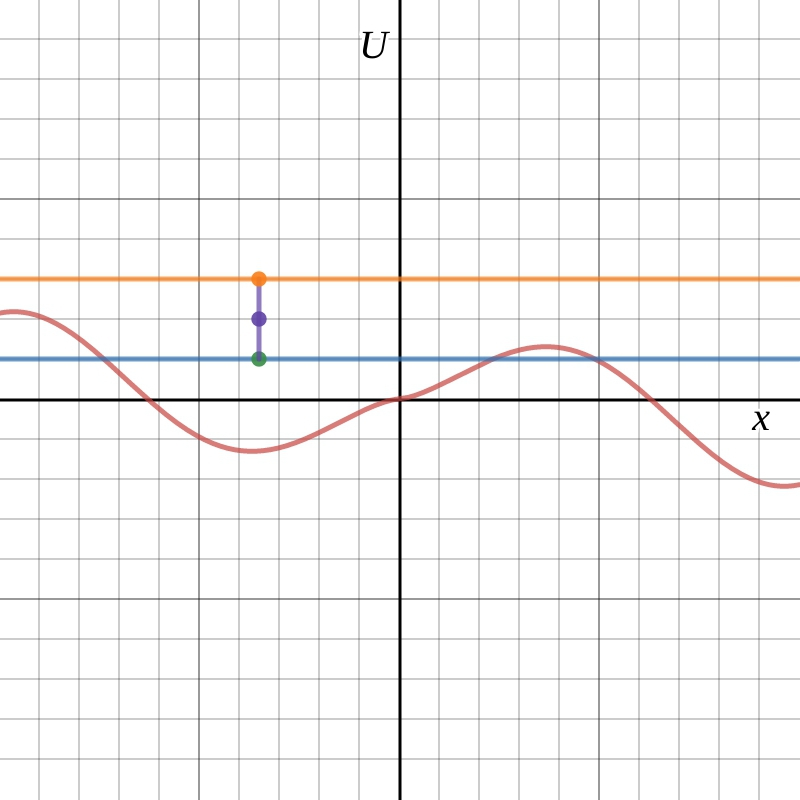
\includegraphics[width=0.4\textwidth]{Appunti/Equilibri.jpg}
    \caption{Esempio di funzione U(x)}
    \label{equilibrienergiapotenziale}
\end{figure}

Nel caso in cui il corpo ha un energia meccanica $E_1$ (quella più bassa) il corpo tende a oscillare intorno al punto di minimo, mentre nel caso $E_2$ (quella più alta) il corpo è altamente instabile e "precipita" cercando il punto di minimo più vicino, per poi oscillarci intorno. Possiamo osservare ciò matematicamente considerando che ogni funzione derivabile due volte in un punto può essere approssimata da una parabola grazie al \textbf{polinomio di Taylor} all'interno della quale il corpo tende a oscillare.

Ritornando alla molla, calcoliamo energia potenziale e cinetica in funzione del tempo nota la soluzione all'equazione differenziale:
\[m\ddot{x}=-k(x-x_0)\then \ddot{y}+\omega y=0\quad\quad \omega=\sqrt{\frac{k}{m}}, y=x-l_0\]
E quindi otteniamo $y=A\sin(\omega t+\phi)$ e sostituendo nelle formule delle energie:
\begin{align*}
    K=\frac{1}{2}m\dot{y}^2=\frac{1}{2}m\omega^2 A^2\cos^2(\omega t+\phi)=\frac{1}{2}kA^2\cos^2(\omega t+\phi)\\
    U=\frac{1}{2}my^2=\frac{1}{2}mA^2\sin^2(\omega t+\phi)
\end{align*}
Quindi l'energia meccanica:
\[E=K+U=\frac{1}{2}kA^2\left(\sin^2(\omega t+\phi)+\cos^2(\omega t+\phi)\right)=\boxed{\frac{1}{2}kA^2}=cost\]
Che ci permette di collegare direttamente l'ampiezza del moto all'energia meccanica del corpo.

\paragraph{Energia Potenziale Gravitazionale}
Noto che $\F_P=m\g=m(0,0,-g)$ allora il lavoro esercitato dalla forza-peso è dato dalla sola componente verticale:
\[\mathbb{L}=-mg\int_{z_1}^{z_2}\dd z=-mg(z_2-z_1)\]
Definiamo quindi l'energia potenziale gravitazionale:
\[U(z)=mgz+c\]
\paragraph{Moto di un Proiettile}
Applichiamo quanto appena dimostrato per la forza-peso al moto di un proiettile, soggetto solo a tale forza:
\[E=\frac{1}{2}mv^2+mgz=\frac{1}{2}m(v_x^2+v_y^2)+mgz\]
Allora note le condizioni iniziali vogliamo calcolare la massima altezza, considerando che l'energia meccanica vale rispettivamete:
\begin{align*}
    E=\frac{1}{2}mv_0^2\\
    E=\frac{1}{2}mv_0^2\cos^2\theta+mgh_M
\end{align*}
Siccoma la forza-peso è conservativa:
\[\frac{1}{2}mv_0^2=\frac{1}{2}mv_0^2\cos\theta+mgh_M\then h_m=\frac{v_0^2-v_0^2\cos^2\theta}{2g}=\frac{v_0^2\sin\theta}{2g}\]
\paragraph{Pendolo}
Similmente al moto del proiettile, l'unica forza a lavoro non nullo agente su un pendolo è la forza peso (in quanto $\tauvt\perp\dd\r$), quindi otteniamo (ponendo il riferimento sul soffitto):
\[E=\frac{1}{2}mv^2+mgz=\frac{1}{2}ml^2\dot{\theta}^2+mgl(1-\cos\theta)\]
Quando raggiunge la posizione massima a $\theta_0$ otteniamo:
\[E=mgl(1-\cos\theta_0)\]
Quindi comparando entrambe le scritture siamo in grado di stabilire un espressione della velocità in funzione dell'angolo/posizione stesso invece che del tempo:
\[\frac{1}{2}ml^2\dot{\theta}^2+mgl(1-\cos\theta)=mgl(1-\cos\theta_0)\then\frac{1}{2}ml^2\dot{\theta}^2=mgl(\cos\theta-\cos\theta_0)\then \dot{\theta}=\sqrt{2\frac{g}{l}(\cos\theta-\cos\theta_0)} \]
Da cui risulta che necessariamente $\cos\theta\leq\cos\theta_0\iff \theta\leq\theta_0$
in $[0,\pi]$.
Possiamo inoltre approssimare per piccole oscillazioni l'energia meccanica del pendolo grazie al polinomio di Taylor:
\[\cos\theta=1-\frac{\theta^2}{2}+o(\theta^4)\then 1-\cos\theta=\frac{\theta^2}{2}+o(\theta^4)\]
Ottenendo:
\[E(\theta)=K(\dot{\theta})+U(\theta)=\frac{1}{2}ml^2\dot{\theta}^2+mgl(1-\cos\theta)\approx\frac{1}{2}ml^2\dot{\theta}^2+mgl\frac{\theta^2}{2}=\boxed{\frac{1}{2}ml[l\dot{\theta}^2+g\theta^2]}\]















\end{document}